%!TeX root=../main.tex
\section{Model} % (fold)
\label{sec:model}

The structure of the data we consider, referred to as \emph{multivariate functional data}, is very similar to that presented in \cite{happMultivariateFunctionalPrincipal2015}. The data consist of independent trajectories of a vector-valued stochastic process $X = (\Xp{1}, \dots, \Xp{P})^\top$, $P\geq 1$. (Here and in the following, for any matrix $A$, $A^\top$ denotes its transpose.) For each $1 \leq p \leq P$, let $\TT{p}$ be a rectangle in some Euclidean space $\RR^{d_p}$ with $d_p \geq 1$, \emph{e.g.}, $\TT{p} = [0,1]^{d_p}$. Each coordinate $X^{(p)} : \TT{p} \rightarrow \RR$ is assumed to belong to  $\sLp{\TT{p}}$, the Hilbert space of squared-integrable real-valued functions defined on $\TT{p}$, having the usual inner product that we denote by $\inLp{\cdot}{\cdot}$, and $\normLp{\cdot}$ the associated norm. Thus $X$ is a stochastic process indexed by $\pointt = (t_1, \ldots, t_P)$ belonging to the $P-$fold Cartesian product $\TT{} : =\TT{1} \times \cdots \times \TT{P}$ and taking values in the $P-$fold Cartesian product space $\HH \coloneqq \sLp{\TT{1}} \times \dots \times \sLp{\TT{P}}$. 

We consider the function $\inH{\cdot}{\cdot} : \HH \times \HH \rightarrow \RR$,
\begin{equation}\label{eq:innerprodH}
    \inH{f}{g} \coloneqq \sum_{p=1}^{P} \inLp{\fp}{\gp} = \sum_{p=1}^{P}\int_{\TT{p}} \fp(t_p)\gp(t_p) \dd t_p, \quad f, g \in \HH.
\end{equation}
$\HH$ is a Hilbert space with respect to the inner product $\inH{\cdot}{\cdot}$\citep{happMultivariateFunctionalPrincipal2015}. We denote by $\normH{\cdot}$, the norm induced by $\inH{\cdot}{\cdot}$. Let $\mu : \TT{} \rightarrow \HH$ denote the mean function of the process $X$, $\mu(\pointt) \coloneqq \EE(X(\pointt)), \pointt \in \TT{}$. Let $C$ denote the $P \times P$ matrix-valued covariance function which, for $\points, \pointt \in \TT{}$, is defined as
\begin{equation}\label{eq:covariance_function}
    C(\points, \pointt) \coloneqq \EE\left(\{X(\points) - \mu(\points)\}\{X(\pointt) - \mu(\pointt)\}^{\top}\right), \quad \points, \pointt \in \TT{}.
\end{equation}
More precisely, for $1 \leq p, q \leq P$, the $(p, q)$th entry of the matrix $C(\points, \pointt)$ is the covariance function between the $p$th and the $q$th components of the process $X$:
\begin{equation}\label{eq:covariance_function_components}
    C_{p, q}(s_p, t_q) \coloneqq \EE\left(\{\Xp{p}(s_p) - \mup{p}(s_p)\}\{\Xp{q}(t_q) - \mup{q}(t_q)\}\right), \quad s_p \in \TT{p}, t_q \in \TT{q}.
\end{equation}
Let $\Gamma : \HH \rightarrow \HH$ denote the covariance operator of $X$, defined as an integral operator with kernel $C$. That is, for $f \in \HH$ and $\pointt \in \TT{}$, the $p$th component of $\Gamma f(\pointt)$ is given by
\begin{equation}\label{eq:covariance_operator_components}
    (\Gamma f)^{(p)}(t_p) \coloneqq \inH{C_{p, \cdot}(t_p, \cdot)}{f(\cdot)} = \inH{C_{\cdot, p}(\cdot, t_p)}{f(\cdot)}, \quad t_p \in \TT{p}.
\end{equation}

Let us consider a set of $N$ curves $\XX = \{X_1, \ldots, X_n, \ldots, X_N\}$ generated as a random sample of the $P$-dimensional stochastic process $X$ with continuous trajectories. Unless otherwise stated, the data are assumed to be observed without error. The data can be viewed as a table with $N$ rows and $P$ columns where each entry is a curve, potentially on a multidimensional domain (see Figure~\ref{fig:data_matrix}). Each row of this matrix represents an observation; while each column represents a functional variable. At the intersection of row $n$ and column $p$, we thus have $\Xnp$ which is the curve that concerns the (functional) feature $p$ for the individual $n$.

\begin{figure}
    \centering
    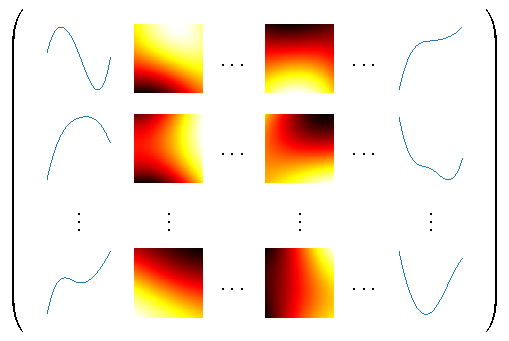
\includegraphics[]{figures/data_matrix.pdf}
    \caption{Functional data matrix, adapted from \cite{berrenderoPrincipalComponentsMultivariate2011}.}
    \label{fig:data_matrix}
\end{figure}

For $n \in \{1, \dots, N\}$, each observation $n$ is attributed the weight $\pi_n$ such that $\sum_n \pi_n = 1$, e.g., $\pi_n = 1/N$.
For a given $p \in \{1, \dots, P\}$, the mean curve of the $p$th component along the $N$ observations is denoted by $\mup{p}$. This quantity can be computed using 
\begin{equation*}\label{eq:mu_estimation}
    \mup{p}(t_p) = \sum_{n = 1}^N \pi_n\Xnp(t_p), \quad t_p \in \TT{p}, \quad p \in \{1, \dots, P\}.
\end{equation*}
The covariance function of the $p$th component along the $N$ observations can be computed using
\begin{equation}\label{eq:cov_estimation}
    C_{p, p}(s_p, t_p) = \sum_{n = 1}^N \pi_n\Xnp(s_p)\Xnp(t_p) - \mup{p}(s_p)\mup{p}(t_p), \quad s_p, t_p \in \TT{p}, \quad p \in \{1, \dots, P\}.
\end{equation}

\subsection{Basis decomposition} % (fold)
\label{sub:basis_decomposition}

% subsection basis_decomposition (end)

In many practical situations, data are noisy and only observed at specific time points. To extract the underlying functional features of the data, smoothing and interpolation techniques are commonly employed. These techniques involve approximating the true curve of the data by finite-dimensional set of basis functions. Assume that for each component $p = 1, \dots, P$, there exists a set of basis of functions $\Psi^{(p)} = \{\psi_k^{(p)}\}_{1 \leq k \leq K_p}$ such that each component of each curve $n = 1, \dots, N$ can be expanded into this basis:
\begin{equation}
\Xnp(t_p) = \sum_{k = 1}^{K_p} c^{(p)}_{nk}\psi_k^{(p)}(t_p), \quad t_p \in \TT{p},
\end{equation}
where $\{c^{(p)}_{nk}\}_{1 \leq k \leq K_p}$ is a set of coefficients for the component $p$ of the curve $n$. We denote by $\overline{c}_k^{(p)} = \sum_{n = 1}^N \pi_n c^{(p)}_{nk}$ the mean coefficient of the component $p$ corresponding to the $k$th basis function along the $N$ curves.
The $p$th component of the mean function can be then expanded in the same basis as:
\begin{equation}
    \mup{p}(t_p) = \sum_{k = 1}^{K_p} \overline{c}_k^{(p)}\psi_k^{(p)}(t_p), \quad t_p \in \TT{p}.
\end{equation}
In a similar way, the covariance function of the $p$th component is given by:
\begin{equation}
    C_{p,p}(s_p, t_p) = \sum_{k = 1}^{K_p} \sum_{l = 1}^{K_p} \left(\sum_{n = 1}^N \pi_n c^{(p)}_{nk}c^{(p)}_{nl} - \overline{c}_k^{(p)}\overline{c}_l^{(p)}\right)\psi_k^{(p)}(s_p)\psi_l^{(p)}(t_p), \quad s_p, t_p \in \TT{p}.
\end{equation}
These formula can be written with a matrix formulation. For $\pointt \in \TT{}$, we have that $X(\pointt) = C\Psi(\pointt)$ where $X(\pointt)$ is a matrix with $N$ rows and $P$ columns with entries $\Xnp(t_p),~t_p \in \TT{p},~1 \leq p \leq P,~1 \leq n \leq N$,
\begin{equation}
    C = \begin{pmatrix}
            C^{(1)} & \cdots & C^{(P)} \\
        \end{pmatrix}, \quad \text{and}\quad
    \Psi(\pointt) = \text{diag}\{\Psi^{(1)}(t_1), \dots, \Psi^{(P)}(t_P)\},
\end{equation}
where
\begin{equation}
C^{(p)} = \begin{pmatrix}
    c^{(p)}_{11} & \cdots & c^{(p)}_{1K_p} \\
    \vdots & \ddots & \vdots \\
    c^{(p)}_{N1} & \cdots & c^{(p)}_{NK_p}
\end{pmatrix} \\
\quad \text{and}\quad
\Psi^{(p)}(t_p) = \begin{pmatrix}
    \psi_1^{(p)}(t_p) \\
    \vdots \\
    \psi_{K_p}^{(p)}(t_p)
\end{pmatrix}.
\end{equation}
Using the basis expansion and denoting $\Pi^\top = (\pi_1, \dots, \pi_N)$, the mean and covariance functions are given by
\begin{equation}
    \mu(\pointt) = \Psi(\pointt)^\top C^\top\Pi \quad\text{and}\quad C(\points, \pointt) = \Psi(\points)^\top C^\top \left(\text{diag}\{
        \pi_1, \dots, \pi_N\} - \Pi\Pi^\top\right)C \Psi(\pointt).
\end{equation}
Finally, we denote by $W$ the matrix of inner products of the functions in the basis $\Psi$. The matrix $W$ is a block-diagonal matrix such that $W = \text{diag}\{W^{(1)}, \dots, W^{(P)}\}$ where each entry is given by
\begin{equation}
    W_{k, l}^{(p)} = \inLp{\psi_k^{(p)}}{\psi_l^{(p)}}, \quad 1 \leq k, l \leq K_p, \quad 1 \leq p \leq P.
\end{equation}
We remark that, if the basis $\Psi$ is an orthonormal basis, the matrix $W$ is equal to the identity matrix of size $\sum_{p = 1}^P K_p$.

% section model (end)